

\begin{figure}
\begin{subfigure}{.5\linewidth}
\centering

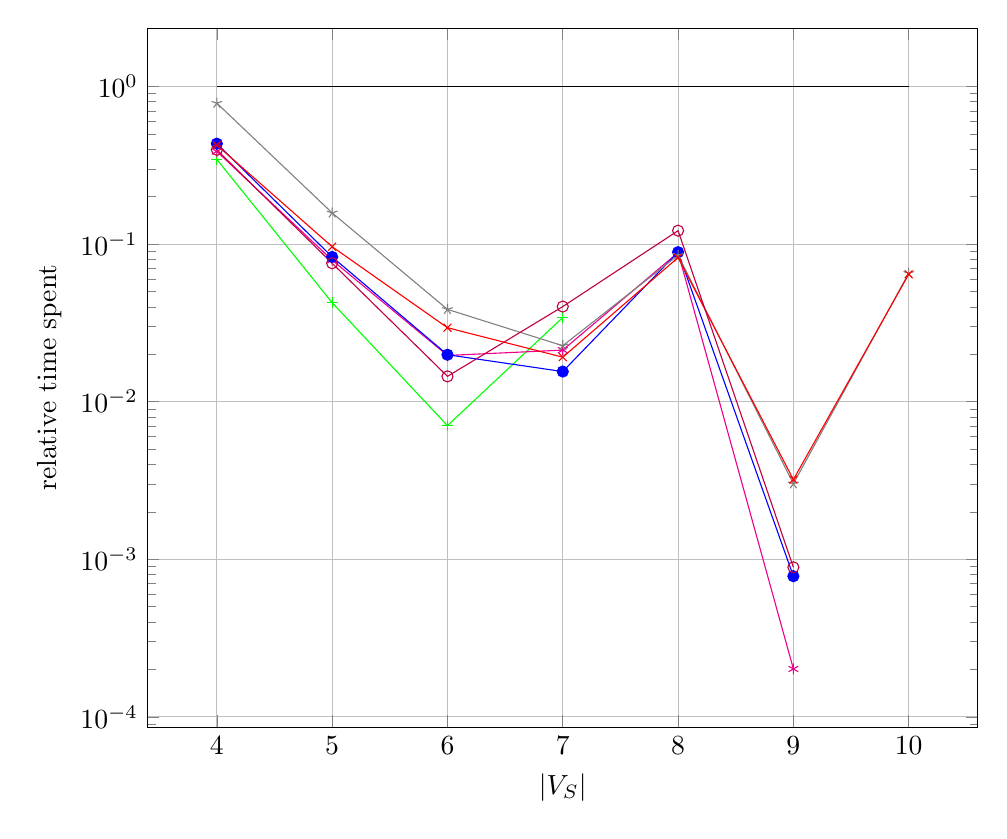
\begin{tikzpicture}
    \begin{axis}[
        xlabel=$|V_S|$,
        ylabel=relative time spent,
        ymode=log,
        legend style={at={(0.9,0.1)},anchor=south east},
        width=\textwidth,
		y tick label style={/pgf/number format/sci},
        ymajorgrids,
        xmajorgrids,		
    ]


\addplot [mark=none, black] plot coordinates {
        (4,1) (10, 1)};
%\addlegendentry{No contraction}
   \addplot[
        mark=+,
        green,
    ] plot coordinates {
        (4,0.34449583915246557)
        (5,0.04250500407360703)
        (6,0.007052140364736389)
        (7,0.034219490143735744)
};
%    \addlegendentry{CP}

\addplot[
        mark=asterisk,
        magenta,
    ] plot coordinates {
        (4,0.38742564587487976)
        (5,0.07909766239343824)
        (6,0.019655091474591525)
        (7,0.021251734957033044)
        (8,0.08842360246711035)
        (9,2.0164236395563237E-4)
};
%    \addlegendentry{GDFS A IP}

\addplot[
        mark=*,
        blue,
    ] plot coordinates {
        (4,0.43377165034858706)
        (5,0.08291766655357158)
        (6,0.019867063872060407)
        (7,0.01553750194233227)
        (8,0.08890227690765527)
        (9,7.816551173891351E-4)
};
%    \addlegendentry{K-Path}

\addplot[
        mark=star,
        gray,
    ] plot coordinates {
        (4,0.7838841422440458)
        (5,0.15772533322419885)
        (6,0.03853822820095056)
        (7,0.02265222193749682)
        (8,0.08504004296545455)
        (9,0.0030177729737449885)
        (10,0.0652985451968477)
};
%    \addlegendentry{GDFS C}

\addplot[
        mark=x,
        red,
    ] plot coordinates {
        (4,0.42425950110101485)
        (5,0.09626130731943527)
        (6,0.029475512058189532)
        (7,0.019168059826692858)
        (8,0.08213870898979722)
        (9,0.00320538172801908)
        (10,0.06429911639723773)
};
%    \addlegendentry{DFS}

\addplot[
        mark=o,
        purple,
    ] plot coordinates {
        (4,0.3963989888723202)
        (5,0.07559274867485685)
        (6,0.014479163749969607)
        (7,0.04015195913379275)
        (8,0.12166475428162647)
        (9,8.901952837352006E-4)
};
%    \addlegendentry{GDFS O IP}


    \end{axis}
    \end{tikzpicture}


\caption{$|V_T|=1\frac{1}{2}*|V_S|$}
\end{subfigure}%
\begin{subfigure}{.5\linewidth}
\centering

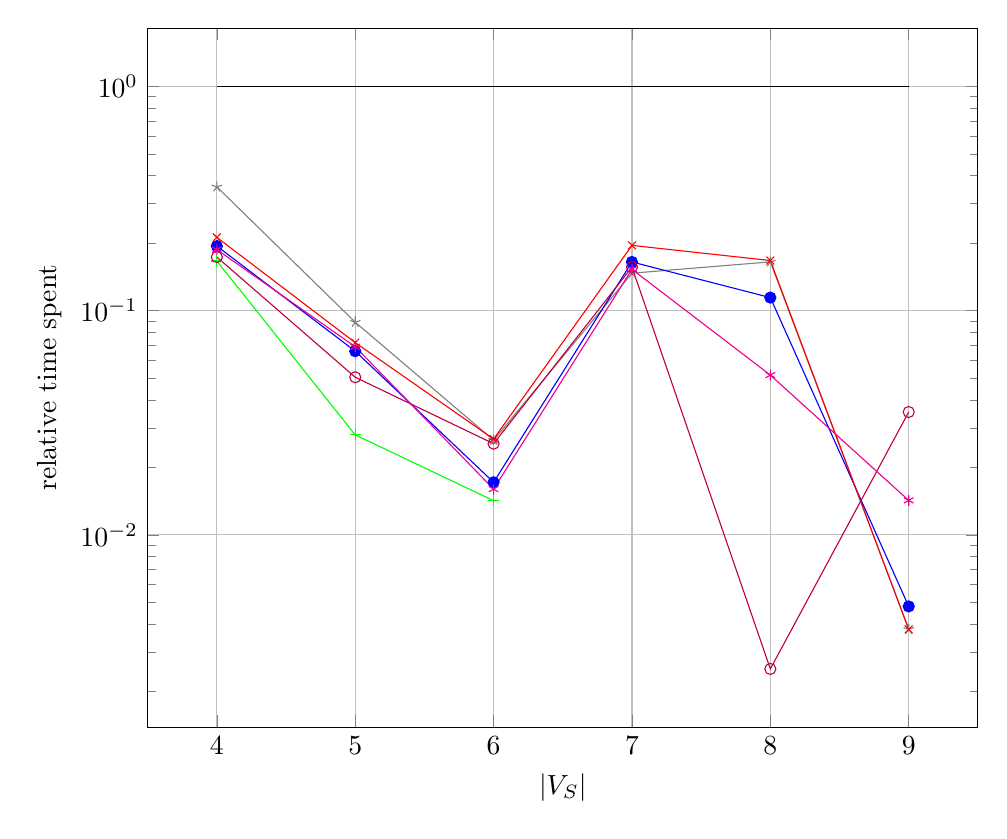
\begin{tikzpicture}
    \begin{axis}[
        xlabel=$|V_S|$,
        ylabel=relative time spent,
        ymode=log,
        legend style={at={(0.9,0.1)},anchor=south east},
        width=\textwidth,
		y tick label style={/pgf/number format/sci},
        ymajorgrids,
        xmajorgrids,		
    ]


\addplot [mark=none, black] plot coordinates {
        (4,1) (9, 1)};
%\addlegendentry{No contraction}

\addplot[
        mark=+,
        green,
    ] plot coordinates {
        (4,0.16656533269519228)
        (5,0.02792481959372131)
        (6,0.014208494420317713)
};
%    \addlegendentry{CP}

\addplot[
        mark=star,
        gray,
    ] plot coordinates {
        (4,0.35670503391181074)
        (5,0.08885285052563148)
        (6,0.02644959281461509)
        (7,0.1469727809071855)
        (8,0.1650715123096471)
        (9,0.003794253797042311)
};
%    \addlegendentry{GDFS C}

\addplot[
        mark=*,
        blue,
    ] plot coordinates {
        (4,0.194158851426724)
        (5,0.06596676865264874)
        (6,0.017166588789163415)
        (7,0.16493104718190343)
        (8,0.11438599305894)
        (9,0.0047972337258095485)
};
%    \addlegendentry{K-Path}

\addplot[
        mark=x,
        red,
    ] plot coordinates {
        (4,0.21233351678836204)
        (5,0.07202295158409817)
        (6,0.026758726043938773)
        (7,0.19551506606564623)
        (8,0.16739005564904727)
        (9,0.003790913734381372)
};
%    \addlegendentry{DFS}

\addplot[
        mark=o,
        purple,
    ] plot coordinates {
        (4,0.17347891126074652)
        (5,0.0504791507537965)
        (6,0.02551664872425517)
        (7,0.15650709939163068)
        (8,0.0025235131787816165)
        (9,0.03532832186507143)
};
%    \addlegendentry{GDFS O IP}

\addplot[
        mark=asterisk,
        magenta,
    ] plot coordinates {
        (4,0.1873514680576187)
        (5,0.06902784077974626)
        (6,0.0160036619729299)
        (7,0.15291763768405797)
        (8,0.0516269965234984)
        (9,0.014247055717867137)
};
%    \addlegendentry{GDFS A IP}
	
	
    \end{axis}
    \end{tikzpicture}

\caption{$|V_T|=3*|V_S|$}
\end{subfigure}\\[1ex]
\begin{subfigure}{0.5\linewidth}
\centering

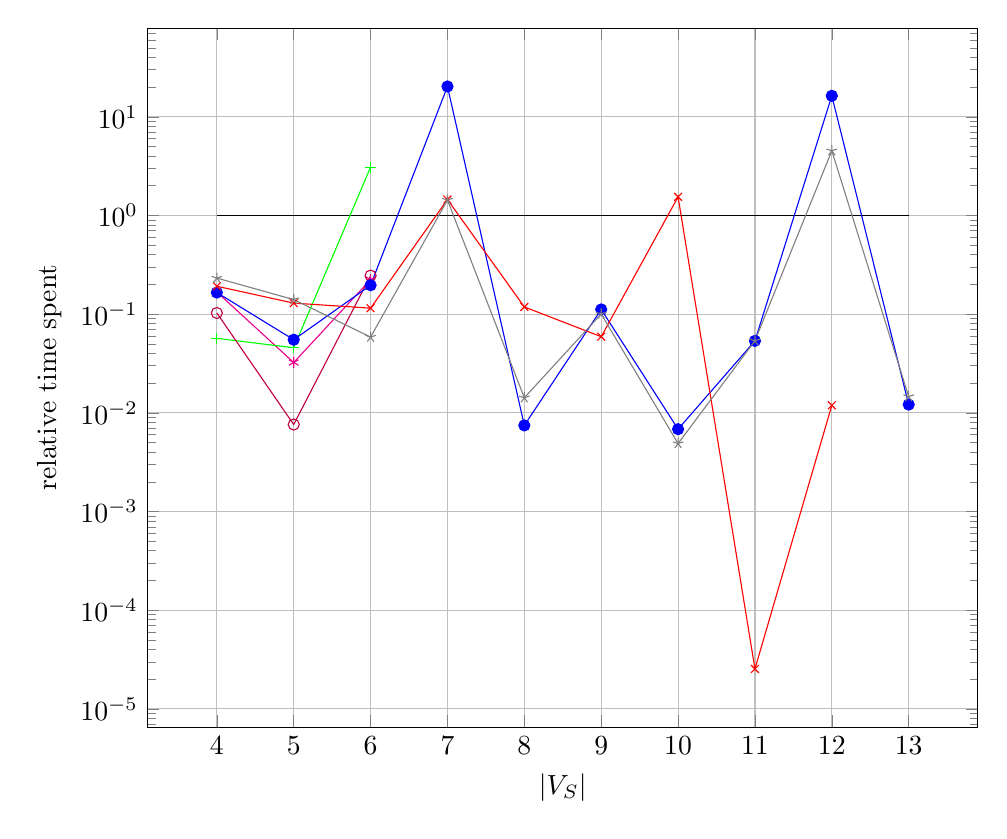
\begin{tikzpicture}
    \begin{axis}[
        xlabel=$|V_S|$,
        ylabel=relative time spent,
        ymode=log,
        legend style={at={(0.9,0.1)},anchor=south east},
        width=\textwidth,
		y tick label style={/pgf/number format/sci},
        ymajorgrids,
        xmajorgrids,		
    ]


\addplot [mark=none, black] plot coordinates {
        (4,1) (13, 1)};
%\addlegendentry{No contraction}

	
\addplot[
        mark=asterisk,
        magenta,
    ] plot coordinates {
        (4,0.1674566113900499)
        (5,0.032349725367020715)
        (6,0.2237865876374895)
};
 %   \addlegendentry{GDFS A IP}
    
    
    \addplot[
        mark=+,
        green,
    ] plot coordinates {
        (4,0.056873208163624955)
        (5,0.04563421043002553)
        (6,3.0895140030860113)
};
 %   \addlegendentry{CP}
    
    \addplot[
        mark=o,
        purple,
    ] plot coordinates {
        (4,0.10276640004366641)
        (5,0.007609829164036706)
        (6,0.24568669245593505)
};
 %   \addlegendentry{GDFS O IP}
    
    \addplot[
        mark=*,
        blue,
    ] plot coordinates {
        (4,0.1655772370426709)
        (5,0.055053818828159615)
        (6,0.19634060714182988)
        (7,20.289869886299307)
        (8,0.007455438509609334)
        (9,0.11168570137538518)
        (10,0.006832180347245251)
        (11,0.053585054708433756)
        (12,16.326793831579934)
        (13,0.01212843469374362)
};
 %   \addlegendentry{K-Path}


\addplot[
        mark=x,
        red,
    ] plot coordinates {
        (4,0.19178983176776473)
        (5,0.1293662743185925)
        (6,0.11496995869605499)
        (7,1.450331503028158)
        (8,0.11835078397595038)
        (9,0.05907513412579321)
        (10,1.545090436667155)
        (11,2.5391954884407796E-5)
        (12,0.011908323973143663)
};
 %   \addlegendentry{DFS}
    
    \addplot[
        mark=star,
        gray,
    ] plot coordinates {
        (4,0.23202692835799185)
        (5,0.14055133962348276)
        (6,0.05857415542176621)
        (7,1.4332274024971468)
        (8,0.014217322662230782)
        (9,0.10041348158626583)
        (10,0.004884744036490124)
        (11,0.053666528274866135)
        (12,4.5260118047084195)
        (13,0.01461043009387195)
};
%    \addlegendentry{GDFS C}
	
	
    \end{axis}
    \end{tikzpicture}

\caption{$|V_T|=5*|V_S|$}
\end{subfigure}
\begin{subfigure} {0.5\linewidth}
\centering

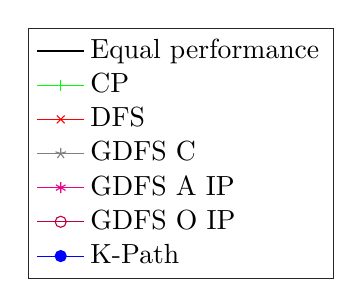
\begin{tikzpicture} 
    \begin{axis}[%
    hide axis,
    xmin=10,
    xmax=50,
    ymin=0,
    ymax=0.4,
    legend style={draw=white!15!black,legend cell align=left}
    ]
	\addlegendimage{black}
    \addlegendentry{Equal performance}; 
     
    \addlegendimage{green, mark=+}
    \addlegendentry{CP};
    
    \addlegendimage{red, mark=x}
    \addlegendentry{DFS};
    
    \addlegendimage{gray, mark=star}
    \addlegendentry{GDFS C};
    
    \addlegendimage{magenta, mark=asterisk}
    \addlegendentry{GDFS A IP};
    
    \addlegendimage{purple, mark=o}
    \addlegendentry{GDFS O IP};
    
    \addlegendimage{blue, mark=*}
    \addlegendentry{K-Path};
    
    \end{axis}
\end{tikzpicture}

\end{subfigure}

\caption{Performance of our algorithm with the GreatestConstrainedFirst source graph vertex order relative to the performance of the algorithm with a random source graph vertex order. ``refuse longer paths" and contraction are disabled and we use no pruning. Data points above the black reference line denote the GreatestConstrainedFirst ordering introduces more delay, and data points below the reference line denote that it saves time. Note the logarithmic y-axis.}	
\label{fig:greatestConstrainedfirstVersusRandom}
\end{figure}


